\graphicspath{{./images/}}

\chapter{Konzepte}

\section{Fachliche Strukturen}

Wie in der Einführung schon erwähnt, geht es bei der Applikation um das Registrieren neuer Händler. Die folgende Abbildung zeigt das Domänenmodell der Applikation. Ziel der Grafik ist es, die Struktur einfach darzustellen weshalb nicht alle Details aufgeführt sind. 

\begin{figure}[H]
	\centering
	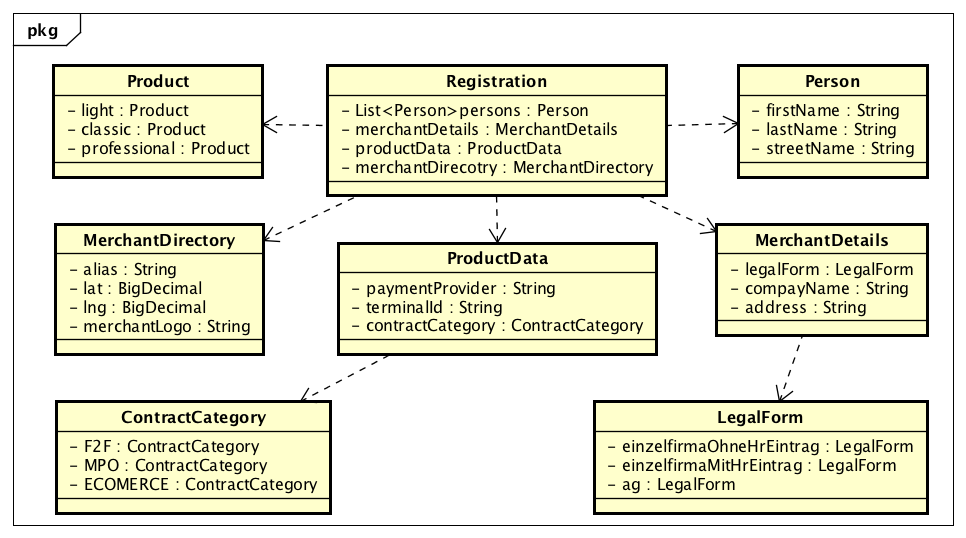
\includegraphics[scale=0.6]{DomainModel.png}
	\caption{Domänenmodell}
\end{figure}

\section{Software Aktualisierung}
\label{software-update}

Die Aktualisierung der Software geschieht mit der neuen Architektur kontinuierlich. Damit dies problemlos funktioniert müssen gewisse Konzepte berücksichtigt werden. Generell sind folgende Regel zu beachten:
\begin{itemize}
	\item Anpassungen müssen rückwärts kompatibel sein. Felder müssen deshalb als 'deprecated' gekennzeichnet werden und sind erst zu entfernen, wenn alle Teil der Applikation aktualisiert wurden.
	\item Mappings auf andere Objekte, wie Datenbank oder Transferobjekte welche an umliegende System geschickt werden, müssen immer mit beiden Versionen funktionieren.
\end{itemize}
Für neue Funktionen welche Änderungen auf mehreren Komponenten zur Folge haben, müssen Feature Toggels verwendet werden. Siehe dazu Kapitel \ref{toggles}.

\subsection{Schnittstellen}

Schnittstellen müssen im Pfad die Versionsnummer enthalten damit der Client die richtigen Endpunkte ansprechen kann. Müssen Änderungen gemacht werden welche sich nicht in die aktuelle Implementierung kombinieren lassen, gilt es, einen neue \textit{\gls{URL}} mit neuer Version zu erstellen. Siehe dazu Kapitel \ref{documents} D-5

\subsection{Persistenz}

Datenbankobjekte müssen wie Schnittstellen ebenfalls rückwärts kompatibel sein, so dass eine kontinuierliche Aktualisierung erfolgen kann. Alte Versionen können nach Bedarf später mittels eines Migrationsskripts auf die neue Version angehoben werden. Das folgende Diagramm zeigt ein Beispiel von Persistenz Klassen wie sie überführt werden. 
\begin{figure}[H]
	\centering
	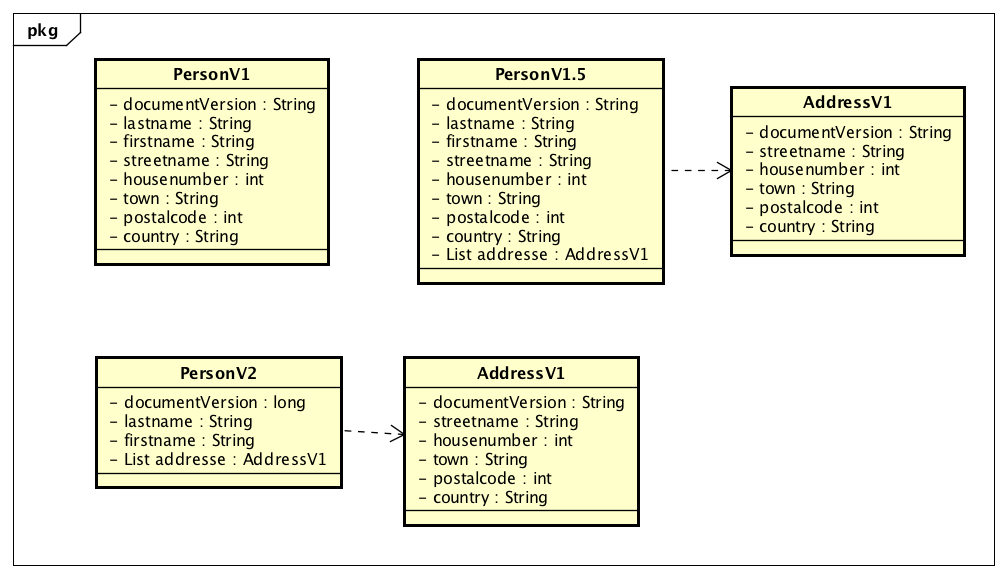
\includegraphics[scale=0.6]{ClassMigration.png}
	\caption{Ablauf der Klassenmigration}
\end{figure}
Die Attribute müssen durch die Service Klassen korrekt abgefüllt werden, so dass während der Aktualisierung die Daten korrekt vorliegen. Weitere Informationen zur Persistenz finden sich in Kapitel \ref{persistenz}.

\section{Typische Muster und Strukturen}

\subsection{Dependency Injection}

Dieser Mechanismus stellt die korrekte Zusammensetzung von Komponenten im Code sicher. Die Abhängigkeiten und Objektinstanzierungen  müssen deshalb nicht durch den Entwickler im Code programmiert werden, sondern das Framework übernimmt diese Aufgabe. Die Basis der Server Applikation bildet Spring Boot. Klassen welche von Spring automatisch iniziert werden sollen, brauchen die passende Annotation.
Damit Spring die Klassen beim Starten findet, muss entweder eine XML oder eine Java Konfiguration des Kontextes vorliegen. Darin werden die entsprechen Packages aufgelistet in welchen gesucht werden soll. Eine ausführliche Erklärung der Funktionsweise findet sich unter \url{https://docs.spring.io/spring/docs/current/spring-framework-reference/html/beans.html}\newline
Im Spring Kontext wird auch oft der Name Beans verwendet wobei diese verschiedene Ausprägungen haben können. In den folgenden Unterkapiteln werden einzelne Ausprägungen genauer erklärt.\newline
Das Web Framework AngularJS verwendet ebenfalls Dependency Injection hat dafür auf Grund der Programmier Sprache JavaScript andere Modelle. Um die Abhängigkeiten aufzulösen können verschiedene Methoden verwendet werden. Eine genaue Erklärung dazu findet sich unter \url{https://docs.angularjs.org/guide/di}

\subsection{Repository}

Repositories sind eine Abstraktionsschicht für die Business Logik welche den Zugriff auf die Datenbank abstrahiert. Sämtliche Operationen zum Speichern, Lesen und Aktualisieren sind über Repositories zu tätigen.  Detaillierte Informationen finden sich unter \url{http://docs.spring.io/spring-data/commons/docs/current/reference/html/}

\subsection{Controller}

Controller dienen als Schnittstelle zwischen einem Web Framework und einer Server Applikation. Dabei werden \textit{\gls{URL}} Pfade auf einem Contollermethode abgebildet und können dadurch von einem Web Client angesprochen werden. Für moderne Applikationen wird als Transportformat \textit{\gls{JSON}} verwendet. Weitere Informationen unter \url{http://docs.spring.io/spring-restdocs/docs/current/reference/html5/}

\subsection{Services}

Serverseitig spricht man bei Services von Klassen welche Business Logik ausführen und somit die Fachlichkeit der Applikation abbilden. Sie befinden sich in einer Schichtenarchitektur zwischen den Controllern und den Repositories. Auf der Frontend Seite sind Services die Abstraktionsschicht welche den Zugriff auf die \textit{\gls{URL}} auf Serverseite kapselt. Siehe auch Kapitel \ref{hystrix}

\subsection{Router}

Für die Navigation zwischen den verschiedenen Web Interface Teilen, wird in AngularJS das Konzept der Router verwendet. Sie definieren die Übergänge zwischen den einzelnen Seiten.

\section{Ausnahme- und Fehlerbehandlung}

Das Applikation hat diverse Schnittstellen zu internen und externen System. Generell wird dabei zwischen zwei Fehlern unterschieden:
\begin{itemize}
	\item Fehler welche korrigiert werden können und somit dem Benutzer nicht angezeigt werden.
	\item Fehler welche nicht korrigiert werden können und somit eine Meldung an den Nutzer zur Folge haben.
\end{itemize}
Die Architektur der Applikation wurde so vorgesehen, dass der Benutzer möglichst keine Fehler des Systems bemerkt. Sämtliche Server sind redundant ausgelegt um eventuelle Netzwerkprobleme, Applikationsabstürze, Installationsprozeduren usw. abzufangen. Siehe dazu auch Kapitel \ref{deploy}. Requests vom Server an die Workflow Engine werden aus diesem Grund asynchron verarbeitet.\newline
Dienste welche nicht von der SIX zu Verfügung gestellt werden, sind meistens auch redundant ausgelegt, ein Fehler muss jedoch mitigiert werden. Dazu zählen die Services des Bundes, Handelsregisters und der Post. Sollte einer der Dienste bei der Registrierung nicht vorhanden sein, muss der Benutzer die Daten manuell ausfüllen und das Risk Management die Daten gegebenenfalls von Hand kontrollieren und erneut freigeben.

\section{Build Management}
\label{build}


Um die Applikation zu bauen und neue Funktionen ausrollen zu können, braucht es eine konfigurierte Build Pipeline. Da bei diesem Projekt GIT zum Einsatz kommt, gibt es mehrere Branches welche den Code für das dazugehörige Stages enthält. Im Generellen gibt es zwei wichtige Branches:
\begin{itemize}
	\item develop: Startpunkt für den Build sowie für die Unit und Integrationstests
	\item master: Enthält den produktiven Code
\end{itemize}
Sämtliche neuen Funktionen und Fehlerbehebungen werden auf einem separaten \textit{\gls{FEBA}} erledigt und erst nach Abschluss in den Development Branch gemerged. Dadurch können die Änderungen unabhängig voneinander durchgeführt werden. Die folgende Grafik zeigt den Ablauf.
\begin{figure}[H]
	\centering
	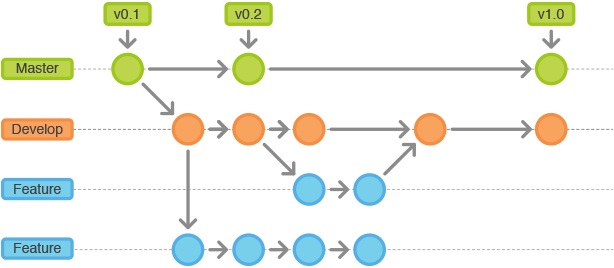
\includegraphics[scale=0.6]{gitflow}
	\caption{GIT Flow Beispiel. Quelle: \url{https://blog.seibert-media.net/blog/2014/03/31/git-workflows-der-gitflow-workflow-teil-1/}}	
\end{figure}
Der Build Job ist als Jenkinsfile eingecheckt und erhält die Beschreibung wie die Pipeline und Ihre Stages definiert sind. Siehe dazu auch \url{https://jenkins.io/doc/book/pipeline/}. Die Pipeline besteht aus verschiedenen Stages welche nacheinander durchlaufen werden so fern es keine Fehler gibt. Für jeden deployment stage gibt es auf OpenShift ein dazugehöriges Projekt in welche die Container ausgerollt werden. Für den finalen Übergang in die produktive Umgebung gibt es einen manuellen Schritt welches ausgeführt wird sobald das Change Management die Änderung bewilligt.

\section{Codegenerierung}

Die AngularJS Services, welche die Anfragen an den Server schicken, werden anhand von Swagger und den RestController automatisch während dem Build Prozess generiert. Sie können durch den Entwickler auch lokal erstellt werden wenn Änderungen gemacht wurden.

\section{Docker Container}
\label{container}
Container, welche vor allem im Zusammenhang mit Docker stehen, sind Software Einheiten mit eigenem Betriebssystem und können auf einen Host wie Linux gestartet werden. Dabei bekommen die Container einen eigenen Bereich auf dem Host System in welchem sie laufen. Dadurch kann Software als Komplettpaket, gegebenenfalls mit zusätzlichen Bibliotheken, ausgerollt werden ohne auf dem Host-System Änderungen machen zu müssen. \newline
Bevor ein Container gestartet werden kann, muss zuerst eine Definition in Form eines Dockerfiles vorliegen. Aus dieser Definition entsteht ein Image welches danach gestartet werden kann und dann als Container läuft. Container sind unveränderlich und verlieren alle Daten welche darin gespeichert wurden. Für diesen Fall wurden persistente Volumen geschaffen welche an einen Container angehängt werden können.

\section{Bedienoberfläche}

Die Benutzeroberfläche wurde mittels des Single Page Application Frameworks AngularJs entwickelt um den Benutzer eine schnelle und einfach zu bedienende Oberfläche zur Verfügung zu stellen. 

\section{Feature Toggles}
\label{toggles}

Toggles erlaubt das Ein- und Ausschalten bestimmter Funktionalitäten einer Software. Ziel ist es, Änderungen welche an einer Anwendung gemacht wurden, erst zu einem späteren Zeitpunkt zu aktivieren. Für den Anwendungsfall von Continuous Deployment ist dies zwingend notwendig, da während der Installation verschieden Versionen der Software am Laufen sind. Neue Funktionen können daher erst aktiviert werden wenn alle Teil der Applikation aktualisiert wurden.

\section{Geschäftsregeln}

Obschon der Serverteil gewisse Fachlogik beinhaltet, werden die Geschäftsregeln auf der Workflow Engine gemacht da nur diese auf die entsprechenden Systeme Zugriff hat. Die Engine basiert auf Camunda und wurde mit eigenen Klassen angereichert um den Prozess der Neuregistrierung für Händler durchzuführen. Der Prozess läuft aus Sicht des Benutzers asynchron ab. Je nach Ausgang sämtlicher Prüfungen und Registrierungen auf den beteiligten Systemen, erhält der neue Händler den Vertrag zugeschickt. Der Anlageprozess läuft generell automatisch ab mit der einzigen Ausnahme, dass die \textit{\gls{PEP}} Prüfung anschlägt. In diesem Fall muss die Risk-Abteilung eine Prüfung durchführen und eine Genehmigung erteilen. Eine weitere Prüfung des Riskbereichs klärt ab, ob der Händler in einem gültigen Geschäftsbereich tätig ist. Sofern dies der Fall ist wird in einem weiteren manuellen Schritt die Auszahlung freigeschaltet.

\section{Internationalisierung}

Das Web Interface ist mehrsprachig ausgelegt und die Sprache kann durch den Benutzer eingestellt werden. Rechtliche Dokumente sind ebenfalls in den entsprechenden Sprachen abgelegt.

\section{Kommunikation, Integration}

Als Kommunikationsmittel zwischen den einzelnen Teilen der Applikation kommen \textit{\gls{REST}} und Messaging zum Einsatz.  \textit{\gls{REST}} ist eine Art um Daten zwischen zwei System auszutauschen. Dabei werden die gängigen HTTP Methoden GET, PUT, POST  verwendet um entsprechende Aktionen auf dem Schnittstelle des Zielsystems auszuführen. Als Übertragungsformat wird  \textit{\gls{JSON}} verwendet.\newline
Das Konfigurationmanagement von Spring Cloud Config verwendet für die Benachrichtigung der Komponenten bei einer Konfigurationsänderung, das Messaging Protokoll  \textit{\gls{AMQP}}. Die Queues werden dabei auf einem separaten RabbitMQ\footnote{Messaging Queue: \url{https://www.rabbitmq.com}} Server gehalten worauf sich der Config Server und die Clients verbinden.

\section{Hystrix}
\label{hystrix}

Hystrix ist eine Bibliothek der Firma Netflix welche für die Kontroller von Anfragen an andere Dienste(\textit{\gls{REST}}, SOAP usw,) verwendet wird. Die Library kümmert sich dabei um Fehlerbehandlung, Wiederholung und Fallback wenn ein Services nicht verfügbar sein sollte. Sämtliche Aufrufe von anderen Diensten innerhalb des Onboarding Server werden mit Hystrix abstrahiert und gekapselt. Siehe auch \url{https://github.com/Netflix/Hystrix/wiki}

\section{Konfiguration}
\label{config}

Die Konfiguration der Applikation besteht aus zwei Teilen. Für die Orchestrierung der Anwendung ist gleichzeitig auch die Deployment Plattform OpenShift zuständig, welche bereits in Kapitel \ref{deploy} vorgestellt wurde. OpenShift verwendet intern Kubernetes für die Koordination der einzelnen Teile. Die sogenannte Deployment Konfiguration basiert auf einer \textit{\gls{YAML}} Datei, welche bei erstellen des Projekt eingelesen werden kann. 
Um die Anwendung  auszurollen benötigt es neben Services und Containern eine Beschreibung wie die Komponenten zusammenhängen. Folgende Konfigurationen müssen gemacht werden:
\begin{itemize}
	\item Docker Image welches verwendet werden soll sowie die verfügbaren Ports und Protokoll.
	\item Persistente Volumen für Datenbank oder Caches.
	\item Services auf welche zugegriffen werden muss. Diese werden dann mittels des internen DNS aufgelöst und eingetragen.
	\item Strategien was bei Konfigurations- und Containeränderungen gemacht werden soll.
	\item Einstellungen für den Gesundheitszustand respektive ob ein Pod noch aktiv ist.
\end{itemize}
Ist die Konfiguration erstellt und in einer Datei gespeichert, kann die Anwendung jederzeit in einem neuen Projekt mit angepassten Parametern ausgerollt werden.\newline
Der zweite Teil bildet Spring Cloud Config womit Konfigurationsänderungen zu Laufzeit ohne Neustart der Applikation möglich sind. Dafür verwendet die Bibliothek einen zentralen Server welcher die Konfigurationen aus einem GIT Repository liest. Die Dateinamen sind nach dem Schema 'applicationname.properties' abgelegt und werden periodisch auf Änderungen überprüft. Die Client Applikation braucht eine Datei 'bootstrap.yml' im Klassenpfad wo der Name der Applikation steht, welche mit dem Namen des Propertyfiles übereinstimmen muss. Dadurch weiss der Config Server welche Einstellungen an die Anwendung zu übermitteln sind. Damit Properties aktualisiert werden, muss die Klasse die Annotation '@RefreshScope' haben. Zusätzlich wird noch ein Bus mittels Queue, basierend auf RabbitMQ, verwendet um die Anwendungen zu benachrichtigen, wenn eine Einstellung geändert hat.

\section{Logging, Protokollierung}

Sämtliche Protokollierungsdaten, welche die Applikation generiert, werden auf die Konsole geschrieben und von dort via OpenShift an den zentralen Splunk Server weitergeleitet.

\section{Management und Administrierbarkeit}

Das Deployment der Applikation kann wahlweise über das Web Interface oder die Konsolenapplikation durchgeführt werden. Die Anwendung selber verfügt über keine Möglichkeiten der Administration. SIX verfolgt mittlerweile den DevOps Ansatz weshalb die Administratoren nicht die Applikation direkt verwalten, sondern sich mehr um die Plattform selber kümmern. Das Management fällt somit dem Entwickler zu. 

\section{Monitoring / Diagnose}

Die Applikation wird einerseits durch OpenShift überwacht mittels Abfragen der Schnittstellen(Liveness Probe) und die Fehlerhaften Teile Notfalls neu gestartet. Zusätzlich hat die Anwendung einen separaten \textit{\gls{REST}} Endpoint welcher Informationen über die einzelnen Dienste bereitstellt. Dies wird erreicht durch die Implementation eines Interfaces welches bei Aufruf zuvor programmierte Aktionen ausführt und die Daten im \textit{\gls{JSON}} Format zurück gibt.

\section{Migration}

Da aktuell als Datenbank MySQL verwendet wird, muss eine Migration nach MongoDB durchgeführt werden. Da die Datenbank nur ein zwischen Speicher ist, müssen nur die Daten der offenen Registrierungen übernommen werden. Da es sich um sechs Tabellen handelt, kann dies mit einem selber geschrieben Tool gemacht werden. MongoDB Inc. bietet dazu einen Guide an wie dies am besten gemacht werden kann. Siehe dazu \url{https://www.mongodb.com/scale/migrate-from-mysql-to-mongodb}.

\section{Persistenz}
\label{persistenz}

\subsection{Datenspeicherung}
Für die Speicherung der Daten wird die \textit{\gls{NoSQL}} Datenbank MongoDB eingesetzt. Anstelle von Tabellen mit einem definierten Schema, werden Dokumente verwendet welche schemalos sind. Dadurch können mehrere Versionen desselben Dokumentes in der Datenbank gespeichert werden. Der Treiber für MongoDB wird beim Mapping nicht vorhandener Attribute, welche sich im Dokument, jedoch nicht auf der Klasse befinden, nicht umwandeln.\newline
Dokumentenklassen in Java müssen ein Attribut haben welches die Version des Dokumentes widerspiegelt. Die Nummer ist bei jeder Änderung der Klasse anzupassen. Dadurch können bei einer Migration die entsprechenden Serviceklassen die Daten gemäss des neuen Dokumentes speichern.

\subsection{Ausfallsicherheit}

Um Ausfallsicherheit zu gewährleisten wird ein Replica Set für die MongoDB aufgebaut. Dabei werden alle Schreiboperationen an den Primary des Set delegiert. Die Replication auf die Secondaries geschieht asynchron. Die folgende Darstellung zeigt den Aufbau:
\begin{figure}[H]
	\centering
	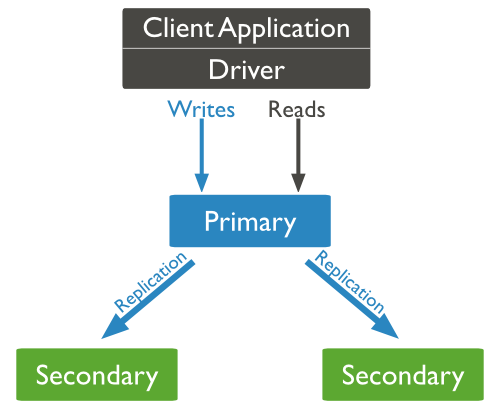
\includegraphics[scale=0.6]{mongodb-replicaset.png}
	\caption{MongoDB ReplicaSet Aufbau. \\ Quelle: \url{https://docs.mongodb.com/manual/replication/}}	
\end{figure}
Im Falle eins Problems mit dem Primary initiieren die Secondaries eine Wahl wer zum neuen Primary wird. Die Instanz, welche einen Fehler hatte, kann neu gestartet werden und sich wieder in das Set einhängen. Sollte ein Knoten des Replica Set länger nicht aktiv sein, wird er 'stale' wodurch die Daten neu synchronisiert werden müssen. Im Kapitel \ref{transactions} finden sich weitere Information bezüglich Transaktionsbehandlung und WriteConcerns.

\section{Plausibilisierung und Validierung}

Auf dem Formular des Web Interfaces sollen Daten wie Händlername via des Unternehmensindentifikationservices des Bundes sowie die Adressen mittels der Services der Post überprüft werden. Angaben, welcher der Händler machen muss, sind entsprechend gekennzeichnet und führen zu einem Fehler falls sie nicht validiert werden können. Der hochgeladene Handelsregisterauszug wird auf der Workflow Engine nochmals mit den, vom Händler eingegebenen Daten abgeglichen.

\section{Sessionbehandlung}

Die Applikation hat ein einmaliges Sessionhandling während der Registrierung eines neuen Händlers. Nach dem ersten Schritt der Registrierung wird ein \textit{\gls{MTAN}} Code und eine Link mittels Mail an den Händer verschickt. Nach dem Klick auf den Link und er korrekten Eingabe des Codes hat der Händler 30 Minuten Zeit um den Prozess abzuschliessen.
Tut er dies nicht, wird die Registrierung abgebrochen und er muss nochmals von vorne beginnen. Ziel der Zeitbegrenzung ist die Verhinderungen von \textit{\gls{DDoS}} Attacken.

\section{Sicherheit}

Die Applikation befindet sich, wie im Kapitel \ref{deploy-dia} dargestellt, in zwei verschiedenen Zonen. Der Teil in der öffentlichen Zone hält keine sensitiven Informationen, welche speziell geschützt werden müssten, sondern Adressdaten der neuen Händler. Diese werden nur kurzzeitig für die Übertragung an die Workflow Engine gespeichert. Der Teil in der PCI Zone steht unter den gleichnamigen Compliance Anforderungen da im gleichen Bereich auch Systeme sind, welche mit Kartendaten arbeiten. Aus diesem Grund ist eine entsprechende Firewall dazwischen. Diese Firewall kann jedoch kein Content Scanning durchführen weshalb vor der Workflow Engine eine Apache WebServer mit einem Security Modul steht. Der Config Server steht ebenfalls in der sicheren Zone um Passwörter zu schützen. Die ganze Kommunikation muss verschlüsselt erfolgen. Durch den Umstieg auf OpenShift ist jedoch noch nicht klar wie die ganzen Zertifikate verwaltet werden resp. ob nur am Eingang ein offizielles verwendet wird oder ob die ganze Kommunikation verschlüsselt sein muss.

\section{Skalierung / Clusterung}

Wie bereits im Kapitel \ref{deploy} angesprochen, können auf der OpenShift Plattform die Anzahl Pods eines Services dynamisch angepasst werden. Dies kann über das WebInterface den OC Client oder über Autoscaling geschehen. Da die Applikation nur wenige tägliche Benutzer hat, wird die Skalierung manuell durchgeführt.

\section{Transaktionsbehandlung}
\label{transactions}
Im Vergleich zu klassischen \textit{\gls{RDBMS}} welche sich an die \textit{\gls{ACID}} Prinzipien halten, hat MongoDB andere Mechanismen wie Transaktionen gehandhabt werden. Schreiboperation welche nur ein einzelnes Dokument aktualisieren sind on MongoBD atomar. WriteConcerns definieren wann MongoDB eine erfolgreiche Speicherung der Daten quittiert. Die zwei vorhandenen Einstellungen sind On-Disk und In-Memory. Um keine Daten zu verlieren wird On-Disk aktiviert.\newline
Da MongoDB als Replica Set aufgebaut wird um einen Ausfall des Primaries zu kompensieren gibt es eine weitere Einstellung mit welcher definiert werden kann, auf wie vielen Replicas der Datensatz ebenfalls gespeichert wird. Für den Anwendungsfall von MEON ist dies nicht notwendig da der Registrierungsprozess mit dem verschicken der SMS Nachricht und der Mail bereits Asynchronität beinhaltet welche genug Zeit für eine Synchronisation der Replicas ermöglicht. Weitere Informationen finden sich in der MongoDB Dokumentation unter \url{https://docs.mongodb.com/manual/reference/write-concern/}.
